
\chapter{The BinaryFile and ArchiveFile classes}
\label{ch-bff}

{\small
\begin{flushright}
Design: Cristina, Mike; Documentation: Cristina, Mike; Implementation: Mike
[c.1997]
\end{flushright}
}

The term "loader" is generally used to describe a system program
used by an operating system (OS) to load a
binary executable file onto memory to execute it. 
We have a class called "BinaryFile" that can be used by application
programs to load other binary files for purposes other than directly
executing them. (The class was formerly called "Loader", but this
contrasts with the use above).
In other words, BinaryFile is a decoder of binary-file formats; it 
reads a binary executable file and stores its representation in memory,
providing functions to access the different parts of the binary
file; such as code and data.  
It provides extra functionality in the presence of 
dynamically linked-in procedures; binary-file formats such as
ELF and PE (Portable Executable) support them.  In this case,
the BinaryFile interface provides a way of determining if a 
procedure address is an address for a dynamically linked-in 
procedure, and if so, it allows access to its code and data.
In this regard, the BinaryFile class is more of a dynamic linker/loader.

Binary files vary widely in internal organisation and structure,
nevertheless, they provide similar kinds of information 
in order to run the program.  
The main components of a binary file are its code and its data;
everything else is a representational structure to access this
information.
By means of the BinaryFile and ArchiveFile classes, we attempt to 
provide a uniform interface for the loading and usage of the 
information stored in binary files.

Some binary file of interest are collected in library or archive
files. The members of the archive are usually object (.o) files;
there is usually a symbol table associated with the archive so that
the member containing the symbol can readily be found. Archive
files are obviously used rather differently than other binary files
(executable and object files), despite attempts to unify them (e.g.
in the elflib library). Therefore, functions for using archive
files are separated into their own class, called ArchiveFile.
(In the previous form, class Loader had a function GetNextMember
to move to the next member of an archive). When a member of the
archive is selected (by index, or procedure name, or file name),
a reference to an instance of a  BinaryFile class is returned, and all the
BinaryFile functions can be called (except for Load; the BinaryFile
object comes "preloaded").


\section{Related Work}
We briefly describe the two main pieces of related work in this
area.

\subsection{GNU's Binary File Descriptor Library}
GNU's Binary-File Descriptor (BFD) Library~\cite{Cham91} is a package
containing common routines that applications can use regardless of 
their underlying binary-file format.
The BFD library divides each specified BFF into the front-end and the
back-end.
The front-end interfaces between the user and the BFD, while
the back-end provides a set of calls which the BFD front-end can use to
decode and manage the object file.
To support a new BFF, the programmer needs to create a new BFD back-end
and add it to the library.
 
BFD has its own binary representation for internal processing known as the
canonical object file format.
When an binary file is opened, the front-end BFD routines automatically 
determine the format of the input file.  A descriptor is built in memory 
with information about which routines are to be used to access
elements of the binary file's data structure.  When the program wants
information about the binary files, the BFD reads from different sections of
the file and processes them.  Each BFD back-end will have routines to convert
section representations of the binary file to BFD's internal canonical
object-file format.
 
The BFD library is provided to the user as a library.  This library
is fairly large; the number of functions offered in the front-end 
are exceptionally many.
The BFD front-end was designed in mind to allow programmers to
be able to retrieve all types of information about \emph{any} BFF; at
least the existing ones at the time.
Due to its generality and bulkiness, it is difficult to use without
spending a big overhead on learning how to use it.
Perhaps because it is too general, it often contain more information 
than is needed for particular system applications.
 

\subsection{SRL - A Simple Retargetable Loader}
SRL, a simple retargetable loader, is a first attempt at developing a 
retargetable loader framework by means of a simple BFF grammar~\cite{Cifu97f}.  
Three different environments, (x86,DOS,EXE), (x86,Windows,NE) and 
(Sparc,Solaris,ELF), were used as the basis for the development and 
testing of SRL.  The three environments gave a good coverage of different 
BFFs currently in use by OSs for RISC and CISC machines. 

The BFF grammar provides support for describing sections of
the binary file, and to name different fields from each section.
Further, it provides support for structures which have been
stored as a sequence of records of a given type, e.g. the number of
elements in the segment table on the NE (New Executable) format,
by means of an array construct -- this construct clearly aids in
the specification of BFFs.

The EBNF for this grammar's syntax is provided in Figure~\ref{fig-bffg}.  
In the grammar, {\it non-terminals} appear in italics, terminals appear in
normal fontface, ``literal strings'' appear with double quotes, and
\verb!examples! appear in courier.
The start symbol for this grammar is {\it BFFspec}.
Hence, the body for any BFF specification is of the form: \\
{\small
{\it spec} $=>$ {\it format-def defin \{defin\} load-info}
}

\centerfigbegin
{\small
\begin{tabular}{lll}
 {\it BFFspec} & $=>$ & {\it \{spec\}}. \\
 {\it spec} & $=>$ & {\it format-def defin \{defin\} load-info} \\
 {\it format-def} & $=>$ & ``DEFINITION'' ``FORMAT'' \\
    & & {\it ident \{ident\}} ``END'' ``FORMAT'' \\
 {\it defin} & $=>$ & ``DEFINITION'' {\it ident} \\
    & & ``ADDRESS'' {\it expression scope-def} \\
    & & ``END'' {\it ident}. \\
 {\it load-info} & $=>$ & ``FILEHEADER'' {\it ident} \\
     & & ``IMAGESIZE'' {\it expression} \\
     & & ``IMAGEADDRESS'' {\it expression} \\
 {\it scope-def} & $=>$ & {\it ident type-exp \{ident type-exp\}} \\
 {\it type-exp} & $=>$ & ``SIZE'' {\it expression} $|$ \\
    & & ``ARRAY'' {\it expression scope-def} \\
    & & ``END'' {\it ident} \\
 {\it expression} & $=>$ & ``('' {\it ident operator expression} ``)'' \\
     & & $|$ {\it ident operator expression} $|$ $\epsilon$ \\
 {\it operator} & $=>$ & ``+'' $|$ ``-'' $|$ ``*'' $|$ ``/'' $|$ ``\^'' $|$ ``\%'' \\
 {\it ident} & $=>$ & ``a''..``z'' $|$ ``A''..``Z'' \{``a''..``z'' $|$ \\
    & & ``A''..``Z'' $|$ ``\_''\} \\
\end{tabular}
}
\centerfigend{fig-bffg}{Binary-File Format Grammar}

SRL, the tool that implements the BFF grammar, was an attempt
to demonstrate the benefit of using a retargetable loader to 
build a machine-code manipulation tool.  SRL was limited in 
a way by its simple grammar which contained a small number of
constructs.  Nevertheless, the BFF grammar was suitable for
specifying most of the sections of the ELF, EXE and NE formats.
SRL generates a C code in the form of a header file (.h) and 
an implementation (.c) file from each parsed file written in
the BFF language.  The header file contains the data structures
needed for the storing of information for a particular
binary file format, and the implementation file provides 
functions for the loading of a file using the structures 
defined in the header file. 


\subsection{Our Approach}
Our approach is different to the two previous ones, as it is more
specific and less retargetable.  We provide an API (via the
BinaryFile class) that 
users must adhere to, but we do not generate code for it automatically
from specifications, nor do we provide for a complete interface
suitable for a large number of binary file formats.  In contrast,
we provide an object oriented abstraction which provides the base
functionality of a loader (regardless of binary file format) in 
an abstract class, and loaders for specific binary file formats 
(e.g. EXE or ELF) inherit from this abstract class and provide new
functionality specific to their format. Similarly, there is an
ArchiveFile class that defines functions for using archive files,
and there are classes derived from this class for the various types
of archive file.


\section{Binary-file formats}
\label{sec-bff}
We briefly describe the abstract format of a binary file.  
Users not familiar with the internal representation of 
binary files who want more detailed information may refer
to the following literature: \cite{Dunc88b,Sun94m,Micr96} and
the web site \url{http://www.wotsit.demon.co.uk} which has a 
compendium of binary file formats.

The general structure of a binary file format (BFF) can be seen to 
be made up by the following abstraction:
\begin{itemize}
\item A header containing general information about the program
and information needed to access various parts of the file.
\item A number of sections holding code and data (raw data).
\item A relocation table containing offsets of relocatable addresses.
\item A symbol table containing information about symbols of the 
	program.
\end{itemize}
Each of these \emph{parts} is given a name respectively: \emph{header},
\emph{sections}, \emph{relocation table} and \emph{symbol table}.
Further, some binary files such as ELF allow for more than one linked
segment to be stored in the one physical file or archive; we refer
to these segments as \emph{members} of the archive.

Most BFFs can be mapped to the general model in Figure~\ref{fig-bffoa};
however, parts are not necessarily stored in that order.
Information regarding the location of sections, symbol tables, etc is
usually identified within the file header.
Nevertheless, some BFFs do not distinguish between these structures; in
the DOS EXE format, the file header contains information about the relocation
table, but there is no information about where the symbol table is stored
(if any), and where data is; there is only one section that embodies all
code, data and symbol table information.
In all cases though, the program's
header will contain enough information to determine the entry point (i.e.
the start of the program's code) in the file.

% Original file in Visio format, on Blimey (in the Drawings directory)
\centerfigbegin
\resizebox{!}{5cm}
{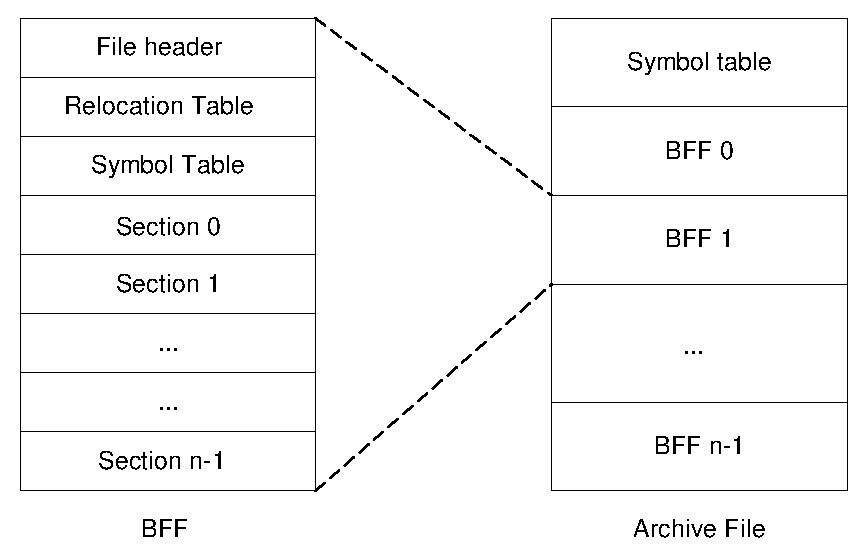
\includegraphics{figures/bffoa.eps}}
\centerfigend{fig-bffoa}{BFF and archive file abstraction}

The current development domain for our tools is based on the Solaris 
ELF~\cite{Sun94m} format, the DOS EXE format~\cite{Dunc88b,Micr96}, 
the Windows (16-bit) NE~\cite{Dunc88b,Micr96} format,
and the Palm OS .prc format~\cite{Tso00}.
Archive files are based on the Unix ar(4) file format.
These formats vary in their degree of complexity and information
stored: the DOS EXE is very simple and limited in structure,
whereas the Solaris ELF format is the most complex, while the Windows
NE is somewhere in between.
The amount of information stored for a simple ``Hello world'' program
varies from format to format.  The DOS EXE format contains a file
header, a relocation table and a single image for both code and data.
The Windows NE version contains most DOS EXE's information plus
additional details such as the resource table, entry table, etc.
The ELF format contains even more information; sections within the 
object file hold information used in dynamic linking: code, data, 
relocation tables, symbol tables, dynamic linking information, etc.
The size in bytes of the binaries for (x86,DOS,EXE), (x86,Windows,NE)
and (Sparc,Solaris,ELF) are 6432, 16384 and 5280 respectively.
It can clearly be seen that although the latter two files are dynamically
linked, their sizes are not necessarily smaller than the static (first)
case.
This is due to the small nature of the example program and the
inclusion of the DOS EXE header information within the NE format.



\section{The BinaryFile Object Hierarchy}
BinaryFile and ArchiveFile are abstract classes; that is, they cannot be
instantiated
directly. The user actually uses classes such as ElfBinaryFile or ExeBinaryFile,
which are derived from the abstract BinaryFile class (see 
Figure~\ref{fig-loadHier}).

% xfig figures exported as eps, portrait, 100% size, displayed at 3.2cm.
\centerfigbegin
\resizebox{!}{3.2cm}
{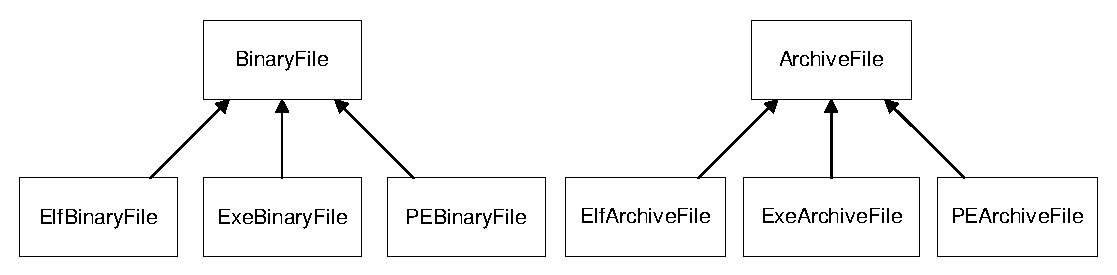
\includegraphics{figures/load_hierarchy.eps}}
\centerfigend{fig-loadHier}{BinaryFile Class Hierarchy}

The user will call functions like \texttt{Load} that are implemented 
differently in the various derived classes. Some functions like
\texttt{SymbolByAddress} are implemented trivially by the BinaryFile class 
(e.g. to always return 0), and this behaviour is overridden by derived 
classes which do the real work.  Even functions like \texttt{GetNumSyms} 
that are implemented by the BinaryFile class will return information that 
will be dependent on the instantiated class.



\section{Interface Functions to Construct and Use a BinaryFile}
The BinaryFile class and each of its parts (described in the abstract 
format description of a binary file in section~\ref{sec-bff}), are 
explained here in terms of interface functions provided for accessing 
information in those parts. 


\subsection{Construction and Loading}
The BinaryFile class provides constructor and destructor 
functions, plus a function to load the binary file.
The loader is an abstract class and hence it does not export 
any types.

\begin{description}
\item [BinaryFile: BOOL $\rightarrow$ BinaryFile].
	This is the constructor. The single BOOL argument is used to
	indicate whether the object to be constructed is to be an
	Archive member; it defaults to false. Users should not use
	this parameter, but should use the ArchiveFile class
	instead (see section~\ref{sec-archive}). The BinaryFile object
	is created without a file loaded; use the Load() function below
	to actually load a file.
	
\item [Load: (BinaryFile x STRING) $\rightarrow$ BOOL].
	Load the given file and store its
	information in a BinaryFile object. It returns whether the
	function was successful or not.
	If there is a problem loading the file, e.g. the file name does
	not exist or there is not enough memory, a message is printed
	on standard error.

\item [UnLoad: BinaryFile $\rightarrow$ nil].
	Deallocates the BinaryFile object. All information about the file
	(e.g. SectionInfo, pointers to section data) are invalid after
	calling this function.

\end{description}


\subsection{Sections}
For each section in the binary file, the following information is 
collected in a SECTIONINFO type:
\begin{itemize}
\item Section name: the name of the section, if any.  Formats like
	ELF support names for each section, such as \texttt{.text} and
    \texttt{.bss}; formats such as EXE do not provide such information
	and hence we follow the convention of naming them \texttt{\.header}
	and \texttt{.text} for the header of the file and the relocatable
	image respectively.

\item Native address: address where the section is logically loaded.
	For example, all EXE files are loaded at address 0x100000,
	representing 10:0000.  ELF files are loaded at the address
	specified in the elf file, typically 0x10000 for code and 0x20000
	for data.  The native address is typically used by diassemblers
	to give a useful address in listing. 

\item Host address: the host address is where the section is actually
	located in virtual memory, i.e. this is a pointer to the first
	byte in the section.

\item Section size: size of the section in bytes.

\item Number of entries: if the section is the equivalent to an 
	array of entries, the size of each entry is given.

\item bCode: This flag is set if the section contains executable
	instructions.

\item bData: This flag is set if the section contains data. It is possible
	for both bCode and bData to be set at the same time.

\item bBss: This flag is set if the section is not initialised, i.e. it
	is for reserving space only.

\item bReadOnly: This flag is set if the section is read only, i.e. it
	cannot be written to.

\end{itemize}

For example, with the ElfBinaryFile class, the section whose name is 
\texttt{\.rodata} would have the flags bData and bReadOnly set.
A disassembler can find all the sections worth disassembling by 
searching through all the sections for those with the flag bCode set.

Sections provide the following functions to determine the number
of sections available in the file and access its information:
\begin{description}
\item [GetNumSections: BinaryFile $\rightarrow$ int].
	Given a BinaryFile object, returns the number of sections that it 
	contains.  

\item [GetSectionInfo: (BinaryFile x int) $\rightarrow$ SECTIONINFO].
	Given an BinaryFile object and a section index, returns the information
	for that section.  Note that sections are indexed from 1.
\end{description}


\subsection{Symbol Table}
Symbol tables are often used for dynamic linking purposes, where
the names of dynamically linked-in routines are stored.  However,
sometimes program symbols are also stored in a symbol table,
whether in the same or a separate table to that of dynamic linking.

The symbol table offered by the BinaryFile class is very simple; 
there are three types of information stored for each entry:
\begin{itemize}
\item Symbol name: the symbol's name in the table.  Type: STRING.

\item Symbol address: the symbol's native address.  Type: ADDRESS.

\item Symbol size: the size in bytes associated with the symbol.
	Type: int.
\end{itemize}

The symbol table offers three access functions to its contents:
\begin{description}
\item [SymbolByAddress: (BinaryFile x ADDRESS) $\rightarrow$ STRING].
	Given a native address, returns the symbolic name associated with the 
	given native address.
	This function is useful when getting names for procedures at
	call locations.

\item [GetAddressByName: (BinaryFile x STRING) $\rightarrow$ ADDRESS].
	Given the name of a symbol, returns the native address associated
	with it.	
	If the symbol is inexistent in the symbol table, an address of 
	0 is returned.

\item [GetSizeByName: (BinaryFile x STRING) $\rightarrow$ int].
	Given the name of a symbol, returns the size in bytes of the 
	symbol, or 0 if inexistent.
\end{description}

Not all BinaryFiles provide the ByName() functions, because in some
cases the binary file format does not support it. If the functions are
not supported, they will always return 0.

Some BinaryFile classes (e.g. ExeBinaryFile) do not implement a symbol table.


\subsection{Relocation Table}
Relocation tables provide information on address that need to be
relocated prior to execution of the program.  
The advantage of knowing which addresses are relocatable is
that when decoding a machine instruction that takes an immediate
operand, we can check if this operand is an address or not. 
This provides us with useful information that is unavailable otherwise.

The functions provided to access the relocation table are:
\begin{description}
\item [IsAddressRelocatable: ADDRESS $\rightarrow$ BOOL].
	Given a native address, returns whether the address is in the
	relocation table or not.

\item [GetRelocatedAddress: ADDRESS $\rightarrow$ ADDRESS].
	Given a native relocatable address, returns the relocated 
	address for it. This function is tentative and not implemented
	as yet; RISC machines require many bit manipulations, and
	this will probably require a different interface function.
\end{description}

With object files, relocations are often associated with symbols.
Sometimes, (e.g. with GCC), intramodule function calls that
could be resolved at compile time are left until link time, so
the call has a relocation entry with an associated symbol table
entry (often not the same symbol table as the main symbols).
To make use of this, the BinaryFile provides this function:

\begin{description}
\item [GetRelocSym: ADDRESS $\rightarrow$ STRING]. Given a
native address, returns a symbol associated with the relocation
at that address, if any. If there is no symbol, the function
returns 0.
\end{description}


\subsection{Program Headers}
Application writers normally like dumping information about 
the headers of the program in order to determine format-specific
information that is not otherwise accessible via the loader
interface.  For example, a loader may have a verbose option to
display this type of information.

Unfortunately, it is difficult to provide a clean interface for
such low level details. (The previous version of the loader
attempted this, but it was not satisfactory). Therefore this
version of BinaryFile provides just one function, for dumping
all the headers in a verbose manner:

\begin{description}
\item [DisplayDetails: BinaryFile x STRING x FILE* $\rightarrow$ BOOL].
	Given a BinaryFile class and the name of the file, sends a verbose
	listing of the
	file to the file indicated by the FILE* parameter.
	The STRING parameter is merely to provide the first line of output,
	which is typically {\it Type} header for {\it Filename}.
	The FILE* parameter can be a special stream such as
	\texttt{stdio}, or a file opened with the \texttt{fopen}
	library function.

\end{description} 

The addresses referred to above are host addresses, i.e. pointers
to actual loaded data. (By contrast, native addresses are those
where part of a file is expected to be loaded in the native
operating system. Headers have no native address.

In the ElfBinaryFile, more specific functions are provided to
access different named headers, such as GetProgramHeader()
and GetSectionHeader().

Given the address of a header, an application writer would have
to know what the contents of the header looks like, and would
have to write the dump function.  We do not consider this
type of detail should be included in our BinaryFile class.


\subsection{Analysis Functions}
The following functions are provided for extra functionality 
required under binary translation, they are:
\begin{description}
\item [GetInitialState: BinaryFile $\rightarrow$ LIST$<$(REGxADDRESS)$>$].
	Returns a list of registers and their initial value (normally
	an address) prior to program execution.

\item [GetEntryPoints: BinaryFile $\rightarrow$ LIST$<$ADDRESS$>$].
	Returns a list of native addresses which are entry points into the 
	program.  The first address is always the initial value of the program
	counter (PC).

\emph{The following function is not implemented at present. It occured to
	me (Mike) that
	the mapping from Native to Host address may vary for each section;
	it doesn't in elf, but it may for other sections. Let's leave this
	one out unless we really need it. It is easy to implement anyway:
	just use the difference between native and host addresses in the
	section info.}
\item [NativeToHostAddress: (BinaryFile x ADDRESS) $\rightarrow$ ADDRESS].
	Given a native address, returns its equivalent host address.
	This function allows access to a block of bytes, since a native
	address is just a pointer.

\item [IsDynamicLinkedProc: (BinaryFile x ADDRESS) $\rightarrow$ BOOL].
	Given a native address, returns whether the address is that of a 
	dynamically linked-in procedure or not in this BinaryFile class.

\item [LoadDynamicLinkedProc: BinaryFile $\rightarrow$ ADDRESS $\rightarrow$ BOOL].
	Given the address of a dynamically linked-in procedure (i.e. the
	target of a call instruction that calls such a function, which
	will usually be an address in the Program Linkage Table), loads
	the appropriate source library file (if needed) to resolve this
	call. It returns its success or otherwise, and the native address
	where the procedure is loaded. 

	There will have to be environment variables to specify what path(s)
	should be searched to locate the appropriate library. These would
	be called \\
	X86\_LIBRARY\_PATH\\
	SPARC\_LIBRARY\_PATH\\
	and so on.  For example,
	if an X86 source program calls the \texttt{atan} function,
	the program's dynamic section specifies the DT\_NEEDED libraries
	as "libc.so.1" and "libm.so.1", and the environment variable
	X86\_LIBRARY\_PATH is set to "/var/lib/x86:/usr/lib/x86", then
	the following libraries will be searched for the \texttt{atan}
	function: \\
	/var/lib/x86/libc.so.1, /var/lib/x86/libm.so.1,
	/usr/lib/x86/libc.so.1, /usr/lib/x86/libc.so.1 \\
	Note that this function is only needed if/when we start supporting
	translations of libraries; at present we assume a native library
	is available.  Hence this function is not implemented at present.
\end{description}



\section{Notes on Individual BinaryFiles}

At present, the ElfBinaryFile is by far the most complete. It is the
only version that implements DisplayDetails(). The need to use
ElfDetails.cc at all, and all the verbose dumping code, can be 
avoided by defining \texttt{NODETAILS} in the make.

The ExeBinaryFile class does not handle symbols (e.g. Microsoft
Codeview or Borland) as these are stored in different ways by
different EXE compilers.

ElfBinaryFile implements symbols, both by address and by name. The
table of symbols looked up by value comes from the \texttt{.symtab}
section, if present, otherwise from the \texttt{.dynsym} section.

When looking up symbols by name, the \texttt{.hash} section is used. This
section refers to the \texttt{.dynsym} section, not the \texttt{.symtab}
section (if present). 
Thus, it is possible to look up local (non dynamic) symbols by value, 
but not by name.  This is a limitation of the way that elf files
are made. 
ElfBinaryFile implements the symbol size field of the SYM\_VALUE passed to 
ValueByName().

Some library files (e.g. libstdc++) have silly dynamic symbol table
entries (that they don't define), with a symbol type of STT\_NOTYPE.
Symbols of this kind are treated as if they don't exist in the symbol
table (i.e. ValueByName() returns 0 for these). 



\section{Interface Functions to Construct and use an ArchiveFile}
\label{sec-archive}

The ArchiveFile class and each of its parts (described in the abstract 
format description of a binary file in section~\ref{sec-bff}), are 
explained here in terms of interface functions provided for accessing 
information in those parts. 

\begin{description}
\item [ArchiveFile: nil $\rightarrow$ ArchiveFile].
	This is the constructor; there are no arguments. The object is
	created without a file being loaded; use the Load function below
	to load an archive file.

\item [Load: STRING $\rightarrow$ BOOL].
	Loads the archive file whose name is given. Returns false if the
	file could not be found, not opened, or it was not an archive
	file. Messages may be displayed on standard error.

\item [UnLoad: ArchiveFile $\rightarrow$ nil].
	Unloads the archive file, and any members that may have been loaded
	and not yet unloaded.  All information about the archive file
	and member files are invalid after calling this function.

\item [GetNumMembers: ArchiveFile $\rightarrow$ int].
	Returns the number of members, not including any special members
	that may exist merely for administrative purposes (e.g. the
	empty members in elf archives that hold the symbol table).

\item [GetMember: ArchiveFile x int $\rightarrow$ BinaryFile*].
	Given an index (0 for first, etc), constructs, loads, and returns
	a pointer to a BinaryFile object for that member. The binaryfile
	object comes pre-loaded; the user should not call the Load function
	for the returned member, but should call UnLoad when done with the
	member object. In the case of errors, a NULL pointer is returned.

\item [GetMemberByProcName: ArchiveFile x STRING $\rightarrow$ BinaryFile*].
	Similar to the above function, except that the relevant member is
	selected by procedure name, e.g. "arctan".

\item [GetMemberByFileName: ArchiveFile x STRING $\rightarrow$ BinaryFile*].
	Similar to the above function, except that the relevant member is
	selected by the name of the archive member (this will usually be an
	object file without an explicit path, e.g. "transcend.o").

\item [GetMemberFileName: ArchiveFile x int $\rightarrow$ STRING].
	Given a member index, return the name of the archive member.


\end{description}

Many of the functions above presume some knowledge of the contents of
the archive, e.g. the file name of the members, or symbols in those
members. There are at present no functions to allow the user to browse
these items.

\section{Example Code}

Examples are often worth a thousand words.  Here are two examples
on how to use the BinaryFile and derived classes.


\subsection{Example 1}
Here is a complete, though simple, program to use the ElfBinaryFile class. 
It simply iterates through the sections of the file, and counts how 
many sections contain code (i.e.  have the ST\_CODE flag set).

\begin{verbatim}
#include <stdio.h>
#include "ElfBinaryFile.h"

int main(int argc, char* argv[])
{
    ElfBinaryFile L;
    int iCnt = 0;

    if (!L.Load(argv[1])) return 1;
    int n = L.GetNumSections();
    PSECTIONINFO pSect = L.GetSectionInfo();
    for (int i=0; i < n; i++)
        if (pSect[i].bCode) iCnt++;
    printf("Part %d has %d code section(s)\n", iPart, iCnt);
    L.UnLoad();
    return 0;
}
\end{verbatim}

This can be compiled as follows (assuming that the above source is in
\texttt{sample.cc}):
\begin{verbatim}
gcc -o sample sample.cc BinaryFile.cc ElfBinaryFile.cc ElfDetails.cc
    SymTab.cc -lelf -lstdc++
\end{verbatim}

The \texttt{"-lelf"} is because ElfBinaryFile requires the elf library; other
versions of the loader would probably not need any libraries other than the
standard template library.
The results are:

\begin{verbatim}
% sample sample
Part 1 has 4 code section(s)

% sample /usr/lib/libelf.a
Part 1 has 1 code section(s)
Part 2 has 1 code section(s)
...
Part 42 has 1 code section(s)
\end{verbatim}


\subsection{Example 2}
The following example dumps the \texttt{\_exit} function
(if present) of the given input file.   Assume the following
code is in file dumptext.cc.

\begin{verbatim}
#include "ElfBinaryFile.h"

int main(int argc, char* argv[])
{
    ElfBinaryFile L;
    SYM_VALUE v;
    PSECTIONINFO pText;

    if (!L.Load(argv[1])) return 1;

    if (L.ValueByName("_exit", &v))
    {
        pText = L.GetSectionInfoByName(".text");
        if (pText)
        {
            int n = v.iSymSize;
            printf("Function _exit (%d bytes):\n", n);
            printf("%08X: ", pText->uNativeAddr);    // Address
            // Compute offset from start of text section to this function
            dword offset = v.uSymAddr - pText->uNativeAddr;
            dword p = pText->uHostAddr + offset;    // Start of function
            for (int i=0; i < n; i++)
                printf("%02X", *((unsigned char*)p++));
            printf("\n");
        }
    }
    else printf("No function '_exit'\n");
    return 0;
}
\end{verbatim}

To compile it, at the command line type:
\begin{verbatim}
gcc -g -o dumpexit dumpexit.cc BinaryFile.cc ElfBinaryFile.cc SymTab.cc 
    ElfDetails.cc -lelf -lstdc++
\end{verbatim}

Sample output: 
\begin{verbatim}
% dumpexit /usr/lib/libc.so.1 
Function _exit (8 bytes):
000169A0: 8210200191D02008
% 
\end{verbatim}

\subsection{Example 3}

The following example loads the archive "/usr/lib/libm.a" and displays
the load address for the "sin" function.

\begin{verbatim}
#include <stdio.h> 
#include "ElfArchiveFile.h"
void main()
{

    ElfArchiveFile af;
    if (!af.Load("/usr/lib/libm.a"))
    {
        printf("ArchiveFile could not load file\n");
        return 1;
    }

    printf("There are %d members in this archive\n", af.GetNumMembers());
    printf("First 5 file names:\n");
    for (int i=0; i < 5; i++)
    {
        printf("%s\n", af.GetMemberFileName(i));
    }

    BinaryFile* pm;
    printf("Object for function 'sin' is at %p\n",
        pm = af.GetMemberByProcName("sin"));
    printf("Address of sin is %p; size %d\n", pm->GetAddressByName("sin"),
        pm->GetSizeByName("sin"));
    pm->UnLoad();

	af.UnLoad();
}
\end{verbatim}

To compile, (assuming the example code is called example3.cc):
\begin{verbatim}
gcc -g -DUNIX -o example3 example3.cc BinaryFile.cc ElfBinaryFile.cc
    SymTab.cc ElfDetails.cc ArchiveFile.cc ElfArchiveFile.cc -lelf -lstdc++
\end{verbatim}


\subsection{Compiling and Linking}
Applications using the BinaryFile class need to compile the files 
\texttt{BinaryFile.cc} and \texttt{ExeBinaryFile.cc} (or \texttt{ElfBinaryFile.cc},
\texttt{PEBinaryFile.cc}, etc).  They should link the resultant object files 
with the application. The final executable must be linked with the standard
template library, e.g. "-lstdc++" for the GCC compiler. Elf versions
also require the elf library, i.e. "-lelf" for GCC.

In addition, BinaryFile classes implementing symbol tables (at present,
this is only the ElfBinaryFile class) also need to compile \texttt{SymTab.cc}
which depends on \texttt{SymTab.h}, and should link with \texttt{SymTab.o}.

For the ElfBinaryFile class, unless \texttt{NODETAILS} is defined in
the make (with \texttt{-DNODETAILS}), the file \texttt{ElfDetails.cc}
must also be compiled and the resultant \texttt{ElfDetails.o} linked.

In those application source files using the BinaryFile class, the appropriate
header file (but not \texttt{BinaryFile.h} itself) should be included. For
example, if using ElfBinaryFile:
\begin{verbatim}
#include "ElfBinaryFile.h"		// Definitions for the ElfBinaryFile class
\end{verbatim}

An example makefile fragment:
\begin{verbatim}
OBJS = myfile1.o ... BinaryFile.o ElfBinaryFile.o SymTab.o ElfDetails.o

ElfBinaryFile.o: BinaryFile.o ElfBinaryFile.h ElfDetails.h

SymTab.o: SymTab.cc SymTab.h

BinaryFile.o: BinaryFile.h
\end{verbatim}



